%version of 07-23-19

\chapter{Numbers I:
The Basics of Our Number System}
\label{ch:numbers-numerals}

\begin{quote}
{\em Let me count the ways} \\
\hspace*{1in}Elizabeth Barrett Browning, ``Sonnets from
the Portuguese'' 43
\end{quote}

\section{Introducing the Three Chapters on Numbers}

Many, perhaps most, of us take for granted the brilliant notations
that have been developed for the many arithmetic constructs that we
use daily.  Our mathematical ancestors have bequeathed us notations
that are not only perspicuous but also convenient for computing and
for discovering and verifying new mathematical truths.  Several
chapters in this text are devoted to sharing the elements of this
legacy with the reader.  Three of these chapters focus on numbers
themselves: the objects and how we represent them.
\begin{enumerate}
\item
This chapter focuses on elementary concepts and techniques of
reasoning relating to the most familiar objects of mathematical
discourse, namely, the four families of numbers that underlie all of
quantitative mathematics.
\item
Chapter~\ref{ch:numbers-advanced} extends this introductory material,
by introducing some more advanced topics concerning numbers.  We look
``inward'' as we discuss important special classes of numbers which
expose deep insights into the intrinsic nature of numbers.  And, we
look ``outward'' as we reveal how numbers can ``encode'' structured
data.  In this latter regard, we suggest some nonobvious implications
of being able to perform such encodings.
\item
Chapter~\ref{ch:numerals} looks at {\it numerals}, \index{numerals}
the strings that we use to manipulate and analyze numbers.
\index{numbers vs.~numerals} We discuss how much one can learn
about various classes of numbers based only on the types of strings
that we can use to name the numbers in the class.
\end{enumerate}

\noindent \fbox{
\begin{minipage}{0.95\textwidth}
Numbers and numerals embody what is certainly the most familiar
instance of a very important dichotomy that pervades our intellectual
lives: the distinction between objects and their names:

\hspace*{.2in}{\em Numbers are intangible, abstract objects.} \index{numbers!as objects}

\hspace*{.2in}{\em Numerals are the names we use to refer to and manipulate numbers.} 
\index{numerals!as names of numbers}

\noindent
This is a critically important distinction!  You can ``touch'' a
numeral: break it into pieces, combine two (or more) numerals via a
large range of operations.  When numerals are {\em operational},
\index{numerals!operational} then you can compute with them.  Numbers are
intangible abstractions, or, conceptualizations: you reason with
numbers.
\end{minipage}
}

\section{A Brief Biography of Our Number System}
\label{sec:number-taxonomy}
\index{number system!biography}
\label{sec:numbers}

We begin our study of numbers and numerals with a short taxonomy of
our number system.  Although we assume that the reader is familiar
with the most common classes of numbers, we do spend some time
highlighting important features of each class, partly, at least, in
the hope of heightening the reader's interest in this most basic
object of mathematical discourse.

We present the four most common classes of numbers in what is almost
certainly the chronological order of their discovery/invention.
%{\Denis the quotation of Kronecker is done 3 times...}

\medskip

\noindent \fbox{
\begin{minipage}{0.96\textwidth}
Did humans {\em invent} these classes of numbers to fill specific
needs, or did we just {\em discover} their pre-existing selves as
needs prompted us to search for them?  The great German mathematician
Leopold Kronecker, \index{Kronecker, Leopold} as
cited in \cite{Weber91} (on page 19), has asserted

\smallskip

\noindent
{\em Die ganzen Zahlen hat der liebe Gott gemacht, alles andere ist
Menschenwerk.}

\smallskip

\noindent
[God made the integers, all else is the work of man].
\end{minipage}
}
\medskip

\noindent
A pleasing narrative can be fabricated to account for our multi-class
system of numbers.  In the beginning, the story goes, we needed to
count things (sheep, bottles of oil, weapons, \ldots), and the
positive {\it integers}\index{number!integer} were discovered to serve
this need.  As accounting practices matured, we needed to augment this
class with the number zero \index{number!zero ($0$)} ($0$) and with the negative integers.
\index{number!negative} 
The former addition (zero) allowed
Merchant $A$ to keep track of the inventory remaining after the last
flask of wine is sold; the latter addition (the negative numbers)
allowed Merchant $A$'s banker to record $A$'s
credit balance after taking a loan.
The class of integers was now complete---although a variety of
special classes of integers remained to be discovered, motivated by
reasons ranging from the religious to the intellectual.

Moving on: As society matured, humans began to share materials that
had to be subdivided---cloth, grain, etc.---rather than partitioned into
discrete units.  We needed to invent the {\it rational numbers}
\index{number!rational} to deal with such materials.  Happily for the
mathematically inclined, the rational numbers could be developed in a
manner that allowed one to view an integer as a special type of rational.
This meant that our ancestors could build upon the systems they had
developed to deal with integers, rather than scrapping those systems
and starting anew.

\medskip

\noindent \fbox{
\begin{minipage}{0.97\textwidth}
{\em This quest for {\em extendible} frameworks rather than isolated
  unrelated frameworks is a hallmark of mathematical thinking.}
\end{minipage}
}
\medskip

\noindent
We now enter the realm of ``semi-recorded'' history in the West: the
Babylonians, the Egyptians, the Greeks, and others.  ``Practical''
mathematics was invented---and reinvented---to accommodate pursuits as
varied as astronomy, commerce, navigation and architecture.  Our
mathematical stalwarts, the integers and the rationals, did not seem
to be able to deal with all of the measurements that we wanted to
make, calculations that we wanted to do, structures that we wanted to
design.  So, we approximated and ``fudged'' and got pretty much where
we wanted to get.  The standard story at this point (at least in the
West) is that the ancient Greeks began to try to systematize
mathematical knowledge and practice.  The Greek mathematician and
geometer Euclid, \index{Euclid} and members of his school,
verified---via one of the first {\em proofs} in recorded history---the
uncomfortable fact that the lengths of portions of eminently buildable
structures were not ``measurable,'' by which they meant {\em not
  rational}.  The poster child for this phenomenon was the hypotenuse
of the isosceles right triangle $T$ with unit-length legs.  Thanks to
the well-known theorem of the Greek mathematician Pythagoras,
\index{Pythagoras} even schoolchildren nowadays know that the length
of this eminently ``buildable'' line is $\sqrt{2}$.  What Euclid
discovered is: {\em There is---provably!---no way to find integers $p$
  and $q$ whose ratio is $\sqrt{2}$, the length of $T$'s
  hypotenuse.}\footnote{We present a version of Euclid's proof in
  Proposition~\ref{thm:sqrt(2)}.}

\medskip

\noindent{\bf $\oplus$ A Digression: The Pythagorean Theorem}.
\index{The Pythagorean Theorem}
The famed Theorem of Pythagoras is widely known, at least informally.
We pause now to provide a {\em formal} statement of this seminal
result and to provide a proof of the special case that relates to our
current discussion of the square-root of $2$.  Quite aside from
reviewing the Theorem's important content, this statement will provide
the reader one more opportunity to ponder the ``music'' of
mathematical discourse.

Let us be given a triangle $T$ with vertices $A$, $B$, and $C$.
\index{triangle} Use the lefthand grey triangle in
Fig.~\ref{fig:unitsquare} as a model.
\begin{figure}[htb]
\begin{center}
       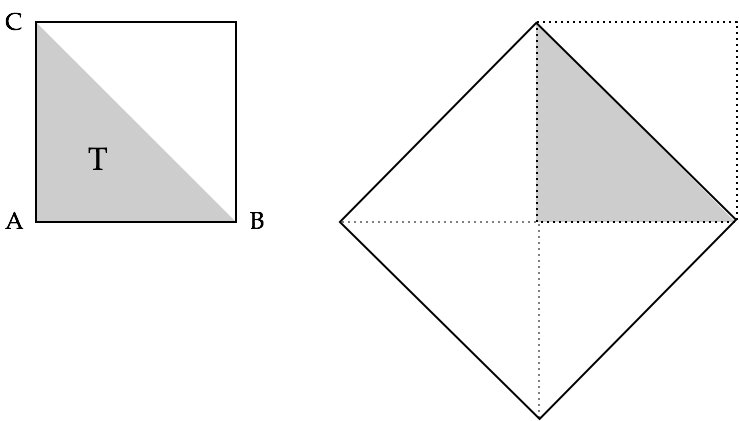
\includegraphics[scale=0.3]{FiguresArithmetic/UnitSquareSQRT2}
\caption{A pictorial schematic proof of The Pythagorian Theorem for
  the special case of an isosceles right triangle.
\label{fig:unitsquare}}
\end{center}
\end{figure}
%
\ignore{\Arny Please edit the figure to follow this story ... label the
  vertices of triangle $T$.  Any other labels? ... hypotenuse?  }
%
Say that $T$ is a {\it right triangle}, \index{triangle!right triangle}
meaning that one of its angles is a {\em right angle},
\index{right angle} i.e., that its measure is $90^\circ$
\index{right angle!$90^\circ$} \index{right angle!$90$ degrees}
\index{right angle!$\pi/2$ radians} 
(read: ``$90$ degrees'') or, equivalently, $\pi/2$ radians.  In our
example, $T$'s right angle occurs at vertex $A$.  Because $T$ is a
right triangle, the line from vertex $A$ to vertex $B$ and the line
from vertex $A$ to vertex $C$ are called the {\em sides}
\index{triangle!right triangle!side}
\index{triangle!right triangle!leg} (or the {\it legs}) of $T$, while
the line from vertex $B$ to vertex $C$ is called the {\em hypotenuse}
\index{triangle!right triangle!hypotenuse} of $T$.  Triangle $T$ is
{\em isosceles} \index{triangle!isosceles triangle} precisely when its
two sides have the same length.  The grey triangle in
Fig.~\ref{fig:unitsquare} is an isosceles right triangle.

\begin{theorem}[{\bf The Pythagorean Theorem}]
\label{thm:Pythagorean-thm}
Let $T$ be a right triangle whose two sides have respective lengths
$s_1$ and $s_2$, and whose hypotenuse has length $h$.  Then
\[ h^2 \ = \ s_1^2 + s_2^2. \]
Consequently, when $T$ is an {\em isosceles} right triangle, then $h^2
= 2 s_1^2$.
\end{theorem}

\ignore{\Denis I put here a figure for proving the result, may be it
  is not at the right place, feel free to put it elsewhere... I
  developed later a graphical proof of the theorem...}

The special case of the Pythagorean Theorem which deals with
isosceles right triangles admits the very perspicuous proof presented
pictorially in Fig.~\ref{fig:unitsquare}.  Let us review this proof.

We begin with the unit-side square $S$ on the left of the figure.  We
partition $S$ by its diagonal into two unit-side isosceles right
triangles, one grey and one white.  In this construction the diagonal
of $S$ is the (common) hypotenuse of the two triangles.  On the
righthand side of Fig.~\ref{fig:unitsquare}, we use our partitioned
version of $S$ to construct a new, bigger square, call it
$\widehat{S}$, whose side-length is the hypotenuse-length of the grey
triangle.  The dotted lines in the figure tell us how big
$\widehat{S}$ is (measured in area).
\begin{itemize}
\item
Square $S$ is unit-sided, hence has unit area.
\item
The grey triangle is (geometrically) half of $S$, hence has area
$1/2$.
\item
Square $\widehat{S}$ is built from four copies of the grey
triangle, hence has area $4 \cdot 1/2 \ = \ 2$.
\end{itemize}
Because the hypotenuse of the grey triangle is a side of an area-$2$
square, we have just proved the following special case of the
Pythagorean Theorem.

\begin{prop}
\label{thm:unit-isosceles-PythThm}
The hypotenuse of the unit-side isosceles right triangle has length
$\sqrt{2}$.
\end{prop}
  
\noindent \textbf{End of digression}

\bigskip
  
As part of the movement toward formalizing mathematics, the
Sicilian-based Greek mathematician and polymath Archimedes \index{Archimedes}
was systematically observing that squares are better approximations to
circles than triangles are; regular pentagons are better than squares;
regular hexagons are better than pentagons; and so on.  
Fig.~\ref{fig:approxcircle} illustrates this evidence.
%
\ignore{\Denis I added a figure here, feel free to remove it if you
  believe it is not appropriate. I can also extend the figure with
  higher degree polygons....} 
\begin{figure}[htb]
\begin{center}
       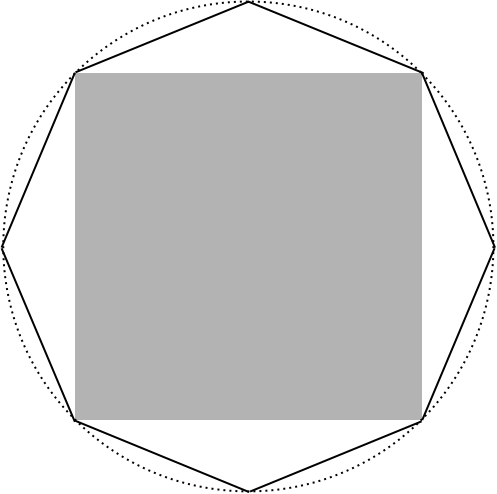
\includegraphics[scale=0.25]{FiguresArithmetic/ApproxCircle}
\caption{{\it Octagons approximate circles much better than squares do.}
\label{fig:approxcircle}}
\end{center}
\end{figure}
In fact, observed Archimedes, as the number of sides, $n$, in a
regular polygon grows without bound (or, as we might say today, tends
to infinity), each increase in $n$ brings a regular polygon closer to
being a circle.

In order to pursue their respective observations to their completion,
both Euclid and Archimedes would have to leave the world of the
rationals and enter the world of the {\it real numbers}
\index{number!real}
(so named by the French mathematician-philosopher Ren\'{e} Descartes).
\index{Descartes, Ren\'{e}}
It would take roughly two-thousand years from the time of Euclid and
Archimedes before the real numbers were {\em formally} introduced to
the world, by mathematical luminaries such as the early-19th-century
French mathematician-scientist Augustin-Louis Cauchy
\index{Cauchy, Augustin-Louis}
and the late-19th-century German mathematician Richard Dedekind.
\index{Dedekind, Richard}
It turned out to be much easier to recognize instances of non-rational
real numbers than to formally delimit the entire family of such
numbers.  Once again, happily, one could develop the real numbers in a
way that allowed one to view a rational number as a special type of
real number.  

During the millennia between the discoveries of Euclid, Archimedes, and
their friends and the full development of the real numbers,
mathematics was enriched repeatedly by the discovery of new conceptual
structures.  One of these---polynomials
\index{polynomial}
and their
\index{polynomial!root}
%
roots---ultimately led to the final major subsystem of our number
system.  In Chapter~\ref{sec:function}, we discussed the important
notion of {\em function}.  Polynomials \index{polynomial} are a
practically important class of functions that are delimited by the
operations needed to compute them.  Specifically, an $n$-argument
polynomial function---typically just called a polynomial---is a
function $P(x_1, x_2, \ldots, x_n)$ whose values can be calculated
using just the basic operations of arithmetic: addition/subtraction
and multiplication/division.\footnote{We pair the operations in this
  way because addition and subtraction are {\em mutually inverse
    operations}, \index{mutually inverse operations} as are
  multiplication and division.  This means that one can undo an
  operation (say, an addition) by performing its inverse operation (in
  this case, a subtraction).  But {\em be careful:} one cannot undo
  multiplication by $0$.}  A {\it root} \index{polynomial!root} of a
polynomial (function) $P(x_1, x_2, \ldots, x_n)$ is an argument
$\langle r_1, r_2, \ldots, r_n \rangle$ that causes $P$ to {\it
  vanish}, meaning that $P(r_1, r_2, \ldots, r_n) = 0$.  In Fig.~\ref{fig:sample-polys},
 \begin{figure}[htb]
\begin{center}
\begin{tabular}{|c|c|c|}
\hline
 & Polynomial $P(x)$ & Root(s) \\
\hline
1 &
$x+1$  &  $x= -1$ \\
2 &
$x-1$  &  $x= 1$ \\
3 &
$x^2 + 2x +1 = (x+1)^2$ & $x = -1$ \\ 
4 &
$x^2 - 2x +1 = (x-1)^2$ & $x = 1$ \\ 
5 &
$x^2 - 1$ & $x = 1$ and $x= -1$ \\
6 &
$x^2 + 1$ & {\em no real root} \\
7 &
$x^2 -2$  & $x = \sqrt{2}$ and $x = - \sqrt{2}$ \\
8 &
$x^2 + 2$ & {\em no real root} \\
\hline
\end{tabular}
\end{center} 
 \caption{A sampler of univariate polynomials.}
 \label{fig:sample-polys}
 \end{figure}
 we illustrate a few sample {\em univariate} (i.e., {\em
  single-variable}) polynomials. \index{polynomial!univariate}\index{polynomial!single-variable}

\medskip

\noindent
There are lessons, both major and minor, to be gleaned from the examples in Fig.~\ref{fig:sample-polys}.

\begin{itemize}
\item
Entries 3 and 4 illustrate that even simple polynomials can often be
written in several different ways.  These entries illustrate also that
roots can occur {\em with multiplicity:}
\index{polynomial!root!multiplicity} one can view the value $x = -1$
as causing the polynomial $x^2 + 2x +1 = (x+1)\cdot (x+1)$ to vanish
in two ways---(1) by setting the lefthand factor $x+1$ to $0$ and (2)
by setting the righthand factor $x+1$ to $0$.

\item
Entries 5 and 7 illustrate that polynomials can have multiple distinct
roots.

\item
Perhaps most importantly, entries 6 and 8 provide explicit, simple
polynomials---whose expressions involve only positive integers---that
fail to have any real roots!

The fact that the indicated polynomials have no real roots is
immediate, because the square of a real number can never be negative.
Hence, for instance, there is no positive integer $c$ such that $c^2 =
-1$, or, equivalently, $c^2 + 1 = 0$.
\end{itemize}

\smallskip

For both applied and purely intellectual reasons, there has always
been considerable interest in developing techniques for finding the
roots of polynomials.  Indeed, much seminal mathematics was developed
in the quest for such techniques;\footnote{A giant in the development
  and transmission of this work was the $9$th-century mathematician
  and astronomer Muhammad ibn Musa al-Khwarizmi \index{al-Khwarizmi,
    Muhammad}.  We describe more about his seminal contributions in
  Chapter~\ref{ch:arithmetic}.}~we study the topic at length in
Section~\ref{sec:polynomials}.

Closely related to this interest in a polynomial's roots was the
considerable discomfort within the mathematical and technical world at
the fact that the then-current number system---built upon the
integers, the rationals, and the reals---was inadequate to the
important task of providing roots for every polynomial.  The reaction
to this deficiency was similar in kind to all earlier recognized
deficiencies: a way was found to expand the number system!  Centuries
would pass before mathematics developed adequately to find the needed
expansion.  Once discovered, the expansion was based in the
conception, in the $16$th century, of a new {\it imaginary} number,
\index{number!imaginary} so designated by \index{Descartes, Ren\'{e}}
Descartes.\footnote{The term ``imaginary'' is reputed to be a
  derogation of these numbers that flouted tradition.}  This new
number was named $i$ \index{imaginary number $i = \sqrt{-1}$}
\index{$i$: the imaginary unit} (for ``imaginary'') and was defined to
be a root of the polynomial $P_{-1}(x) = x^2 +1$.  The number $i$ was
evocatively often defined via the equation, $i = \sqrt{-1}$.  By
keeping our extended arithmetic consistent with our former arithmetic,
$-i$ also became a root of $P_{-1}(x)$.  When the imaginary number $i$
was added to the real number system, and the combination was blended
via the rules of arithmetic, the {\it complex number
  system}\index{number!complex} was born.

Thankfully, the imaginary number $i$ was the only totally new concept
that was needed to mend the observed deficiency in the real numbers.
In formal terms, the complex numbers were shown to be {\it
  algebraically complete} \index{complex numbers!algebraically
  complete} in the sense expressed in the landmark {\it Fundamental
  Theorem of Algebra}: \index{Fundamental Theorem of Algebra}

\begin{theorem}[The Fundamental Theorem of Algebra]
Every polynomial of degree $n$ with complex coefficients has $n$ roots
over the complex numbers.
\end{theorem}

The proof of the Theorem is beyond the scope of our introductory text,
but the result is a notable milestone in our mathematical/technical
culture.

\medskip

Our historical tour is now complete, so we can---finally---begin to
get acquainted with the several components our number system and the operations that bring
each component to life in applications.

\section{Integers: The ``Whole'' Numbers}
\label{sec:integers}

The most basic class of numbers are the {\it integers},
\index{number!integer}
which are also referred to as the {\it whole numbers}
\index{number!integer!whole number}
or the {\em counting numbers}.
\index{number!integer!counting number}
%
As suggested in our ``biography'' of our number system
(Section~\ref{sec:number-taxonomy}), integers are certainly the
numbers that our prehistoric ancestors employed in the earliest days
of our species.  This section is devoted to exploring some of the
basic properties of the class of integers.  The details we provide in
Section~\ref{sec:primes} regarding the building blocks of the
integers, the {\it prime numbers}, \index{number!prime} will prepare
the reader for myriad applications of the integers, including
important {\em (computer-)security-related} applications.  Our introduction to {\it
  pairing functions}, \index{pairing functions} in
Section~\ref{sec:pairing}, will open the door to myriad
applications of the integers that build on the ordering properties of
these numbers, coupled with tools for encoding highly structured data
as integers.

\subsection{The Basics of the Integers: The Number Line}
\label{sec:integer-number-line}
\index{number!the number line}
\index{number!integer!the number line}

We survey a number of the most important properties of the following
three sets, which collectively comprise ``the integers.''
\begin{itemize}
\item
The set $\Z$
\index{$\Z$: the set of all integers}
comprises {\em all integers}---the positive and negative integers and
zero ($0$).
\item
The set $\N$
\index{$\N$: the set of nonnegative integers}
comprises the {\em nonnegative integers}---the positive integers and
zero ($0$).
\item
The set $\N^+$
\index{$\N^+$: the set of positive integers}
comprises the {\em positive integers}.
\end{itemize}
There is no universal default when one refers to ``the integers'' with
no qualifying adjective; therefore, we shall always be careful to
indicate which set we are discussing at any moment---often by
supplying the set-name: $\Z$ or $\N$ or $\N^+$.

\subsubsection{Natural orderings of the integers}
\label{sec:natural-orderings}

Several essential properties of the sets $\Z$, $\N$, and $\N^+$ are
consequences of the integers' behaviors under their natural order
relations:
\begin{itemize}
\item
the two {\em less-than} relations:
  \begin{itemize}
  \item
the {\em strict} relation ($<$).  We articulate ``$a < b$'' as ``$a$
is (strictly) less than $b$'' or ``$a$ is (strictly) smaller than
$b$.''
  \item
the {\em nonstrict} relation ($\leq$).  We articulate ``$a \leq b$''
as ``$a$ is less than or equal to $b$'' or ``$a$ is no larger than
$b$.''
  \end{itemize}
\index{$<$: the strict less-than relation} \index{$\leq$: the nonstrict less-than relation}

\item
their {\em converses,} the {\em greater-than} relations:
  \begin{itemize}
  \item
the {\em strict} relation ($>$).  We articulate ``$a > b$'' as ``$a$
is (strictly) larger than $b$.''
  \item
the {\em nonstrict} relation ($\geq$).  We articulate ``$a \geq b$''
as ``$a$ is greater than or equal to $b$'' or ``$a$ is no smaller than
$b$.''
  \end{itemize}
\index{$>$: the strict greater-than relation}
\index{$\geq$: the nonstrict greater-than relation}
\end{itemize}
One sometimes encounters {\em emphatic} versions of the strict
relations: $a << b$ and $a >> b$ indicate that $a$ is, respectively,
{\em much smaller than} or {\em much larger than} $b$.
\index{$<<$: the emphatic strict less-than relation}
\index{$>>$: the emphatic strict greater-than relation}

The reader will note throughout the text that order within a number
system is among one's biggest friends when reasoning about the numbers
within the system.  \index{number!ordering of numbers}

\subsubsection{The order-related laws of the integers}
\label{sec:order-laws}

\noindent{\small\sf A. Total order and the Trichotomy Laws}

The sets $\Z$, $\N$, and $\N^+$ are {\em totally ordered},
\index{number!integer!total order}
\index{integer!total order}
also termed {\em linearly ordered}
\index{number!integer!linear ordering}
\index{integer!linear ordering}.
\smallskip

These facts are embodied in the {\em Trichotomy Laws for integers}.
\index{number!integer!Trichotomy Laws}
\index{integer!Trichotomy Laws}
\index{Trichotomy Laws}
\medskip

{\it The Trichotomy Laws for integers}.
\smallskip

(i)
%
{\it For each integer $a \in \Z$, precisely one of the following is true.}

\hspace*{.2in} $a$ equals $0$: $(a=0)$ \ \ \ \ \ \
 $a$ is {\em positive}: $(a>0)$ \ \ \ \ \ \
 $a$ is {\em negative}: $(a<0)$
\smallskip

(ii)
%
{\it For each integer $a \in \N$, precisely one of the following is true.}

\hspace*{.2in} $a$ equals $0$: $(a=0)$ \ \ \ \ \ \
 $a$ is {\em positive}: $(a>0)$
\smallskip

(iii)
%
{\it For each integer $a \in \N^+$:}

\hspace*{.2in} $a$ is {\em positive}: $(a>0)$
\bigskip

Consequently:
\smallskip

(i')
$\Z$ can be visualized via the ($2$-way infinite) number line:
\index{number!the number line}
\[ \ldots, -3, \  -2, \ -1, \ 0, \ 1,\  2, \ldots \]
\smallskip

(ii')
$\N$ can be visualized via the ($1$-way infinite) number line:
\[  0, \ 1, \ 2, \ 3, \ldots \]
\smallskip

(iii')
$\N^+$ can be visualized via the ($1$-way infinite) number line:
\[  1, \ 2, \ 3, \ldots \]
\bigskip

The Trichotomy Laws can be expressed using arbitrary pairs of integers,
rather than insisting that one of the integers be zero.  For the set
$\Z$, for instance, this version of the Laws takes the following form:

{\it For any integers $a, b \in \Z$, precisely one of the following is
  true.}

\hspace*{.2in} $a$ equals $b$: $(a=b)$ \ \ \ \ \ \
 $a$ is less than $b$: $(a<b)$ \ \ \ \ \ \
 $a$ is greater than $b$: $(a>b)$

\medskip

\noindent{\small\sf B. Well-ordering}

The sets $\N$ and $\N^+$ are {\it well-ordered}.
\index{number!nonnegative integers!well-ordering}
\index{nonnegative integers!well-ordering}
\index{number!positive integers!well-ordering}
\index{positive integers!well-ordering}
\medskip

\noindent
{\it The Well-ordering law for nonnegative and positive integers}. \\
%
{\it Every subset of $\N$ or of $\N^+$ has a smallest element (under
  the ordering $<$).}

\medskip

\noindent{\small\sf C. Discreteness}

The set $\Z$ is {\it discrete}.
\index{number!integer!discreteness}
\index{integer!discreteness}
\medskip

\noindent
{\it The discreteness of the integers.} \\
%
{\it For every integer $a \in \Z$, there is no integer between $a$ and
  $a+1$; i.e., there is no $b \in \Z$ such that $a < b < a+1$.}

\medskip

\noindent{\small\sf D. The law of ``between-ness''}

{\it The ``between-ness'' law} for the set $\Z$:
\index{number!integer!''between-ness'' law}\index{integer!''between-ness'' law}
\smallskip

\noindent
{\it For any integers $a, b \in \Z$, there are finitely many $c \in
  \Z$ such that $a < c < b$.}
\smallskip

\noindent
Any such $c$ lies {\em between} $a$ and $b$ along the number
line, whence the name of the law.

\medskip

\noindent{\small\sf E. The cancellation laws}

There are two {\it cancellation laws} for the set $\Z$,
\index{number!integer!cancellation laws}
\index{integer!cancellation laws} one for the operation of addition
and one for the operation of multiplication.
\medskip

\noindent
{\it The cancellation law for addition}. \\
%
{\it For any integers $a, b, c \in \Z$, if $a+c = b+c$, then $a = b$.}
\index{number!integer!cancellation laws!addition}
\index{integer!cancellation laws!addition}
\smallskip

\noindent
{\it The cancellation law for multiplication}. \\
%
{\it For any integers $a, b \in \Z$ and $c \in \Z \setminus \{0\}$, if
  $a \cdot c = b \cdot c$, then $a = b$.}
\index{number!integer!cancellation laws!multiplication}
\index{integer!cancellation laws!multiplication}
\smallskip

\noindent
The cancellation laws provide limited versions of the algebraic notion
of mutually inverse arithmetic operations
(Section~\ref{sec:binary-operators}).
\index{arithmetic operations!mutually inverse operations}


\subsection{Divisibility: Quotients, Remainders, Divisors}
\label{sec:divisibility}
\index{divisibility}
\index{integers!divisibility}

This section is devoted to studying the fundamental relation of {\em
  divisibility} between two integers.  Let $m, n \in \N$ be
nonnegative integers.  We use any of the following locutions to assert
the existence of a positive integer $q$ such that $n = q \cdot m$.
\index{number!integer!divisor}
\index{number!integer!divisibility}\index{$m \mid n$: $m$ divides $n$}
\begin{itemize}
\item
$m$ {\it divides} $n$
\item
$m$ {\it is a divisor of} $n$
\item
$n$ {\it is divisible by} $m$
\item
$m \mid n$.
\end{itemize}
This section is devoted to studying the possible {\it divisibility}
relations between integers $m$ and $n$.  We begin by noting some
general facts.
\begin{itemize}
\item
{\em Every integer $m$ divides $0$.}

This is because of the universal equations $m \cdot 0 = 0 \cdot m = 0$.  
The same equations verify that $0$ {\em does not divide any integer.}

\item
{\em $1$ divides every integer.}

This is because of the universal equation $1 \cdot m = m$.
\item
{\em Every nonzero integer divides itself.}

This is because of the universal equation $m \cdot 1 = m$.
\end{itemize}

Some nonzero integers have many distinct divisors, while some have
very few.  Consider, for illustration, the first twelve positive
integers.
\[ \begin{array}{|c|c|}
\hline
\mbox{Number} & \mbox{Divisors} \\
\hline
\hline
1  &  \{ 1 \} \\
2  &  \{ 1, 2 \} \\
3  &  \{ 1, 3 \} \\
4  &  \{ 1, 2, 4 \} \\
5  &  \{ 1, 5 \} \\
6  &  \{ 1, 2, 3 \} \\
7  &  \{ 1, 7 \} \\
8  &  \{ 1, 2, 4, 8 \} \\
9  &  \{ 1, 3, 9 \} \\
10  & \{ 1, 2, 5, 10 \} \\
11  & \{ 1, 11 \} \\
12  & \{ 1, 2, 3, 4, 6, 12 \} \\
\hline
\end{array}
\]
All nonzero integers (but 1) have at least two divisors, $1$ and themselves.
The ``sparsely divisible'' integers that have only these two divisors
are called {\it primes}\index{numbers!integers!prime} or {\it prime
  integers} or {\it prime numbers}.  We study these ``building blocks
of the positive integers'' in more detail in Section~\ref{sec:primes}.
While there is, indeed, much of interest to discuss about prime
numbers, the \index{numbers!integers!composite} {\it composite}---or,
nonprime---integers are also quite interesting, particularly, when we
focus of {\em pairs} of integers.  The next section looks at the
defining property of composite integers, namely, {\em divisibility}.

\medskip

In order to better understand the fundamental concept of divisibility,
we must broaden our perspective somewhat and consider the notion of
{\em Euclidean division}, \index{Euclidean division} i.e., division
with remainders.  The notion of ``perfect'' divisibility that we have
been discussing thus far is the special case in which the remainder is
$0$.  The next subsection studies Euclidean division; the remainder of
this section investigates the ramifications of ``perfect''
divisibility.

\subsubsection{Euclidian division}
\label{sec:euclidian}
\index{Euclidean division}

Divisibility is not always perfect: Given a pair of integers, neither
needs be an integer multiple of the other.  As we learned in
elementary school, if an integer $m > 0$ does not ``evenly'' divide an
integer $n > m$, then we are left with a ``remainder'' when we attempt
to divide $n$ by $m$.  {it Euclidean} \index{Euclidean division} {\it
  division}---so named for the Greek mathematician Euclid,
\index{Euclid} whose writings introduced the process in the West---is
the process of producing, given integers $m >0$ and $n >m$, an integer
{\it quotient} \index{quotient} $q$ and an integer {\it remainder}
\index{remainder} $r$ (where $0 \leq r < m$) such that $n = q \cdot m
+ r$.  The process of Euclidean division always succeeds, in the
following strong sense.

\begin{prop}[The Division Theorem]
\label{thm:division-thm}
Given any integers $n$ and $m > 0$, there exists a unique pair of
integers $q$ and $r$, with $0 \leq r < m$ such that
\begin{equation}
\label{eq:euclid-division}
n \ = \ q \cdot m + r.
\end{equation}
\end{prop}

\begin{proof}
We first prove that a result-pair $\langle q, r \rangle$, as described
in the Proposition, exists for each argument-pair $\langle m, n
\rangle$.  Then we prove that the result-pair is unique.

\medskip

\noindent {\em There exists at least one argument-pair}.
%
Given any argument-pair $\langle m, n \rangle$, let $N_{m,n}$ be the
set of all integers of the form $(n - a \cdot m)$ for some
integer $a$.  Symbolically,
\[ N_{m,n} \ \eqdef \ \{ (n - a \cdot m) \ \ | \ \  \mbox{ both } \  a,  \
(n - a \cdot m) \in \N  \}
\]

Each such set $N_{m,n}$ is a nonempty set of nonnegative integers: the
nonemptiness follows because $n \in N_{m,n}$ (via the case $a=0$).  By
the Well-ordering law, $N_{m,n}$ contains a (perforce, unique) {\em
  smallest} element.  Let us denote this smallest element by $r$, and
let us denote by $a_r$ the value of $a$ that yields $r$; i.e.,
\[ n - a_r \cdot m \ = \ r.  \]
We complete this section of the proof, we need show that $r < m$.
Say, for contradiction, that $r = m+r'$ for some $r' \in \N^+$.  We
then find
\[ n - (a_r +1)  \cdot m \ = \ r -m \ = r' \]
to be an element of $N_{m,n}$ that is strictly smaller than $r$.  This
contradiction completes the first part of the proof.
\medskip

\noindent {\em 2. There exists at most one argument-pair}.
%
Turn now to the issue of uniqueness.  Say, for the sake of
contradiction, that there exists an argument-pair $\langle m, n
\rangle$, for which there exist distinct result-pairs $\langle q_1,
r_1 \rangle$ and $\langle q_2, r_2 \rangle$.  We therefore have
\begin{equation}
\label{eq:euclid-unique}
n \ = \ q_1 \cdot m + r_1 \ = \ q_2 \cdot m + r_2,
\end{equation}
where both $r_1$ and $r_2$ satisfy the inequalities $0 \leq r_1, r_2
<m$.  We consider two cases.
\begin{itemize}
\item \textbf{Case 1.}
Assume first that $r_2 = r_1$.  In this case, the equations
(\ref{eq:euclid-unique}) tell us that
\[ q_1 \cdot m \ = \ q_2 \cdot m. \]
The cancellation law for multiplication then tells us that $q_1 =
q_2$.  Therefore, the allegedly distinct result-pairs are, in fact,
identical.

\item \textbf{Case 2.}
If $r_2 \neq r_1$, then say, with no loss of generality, that $r_2 >
r_1$.  In this case, the equations (\ref{eq:euclid-unique}) tell us
that
\[ (q_1 - q_2) m \ = \ r_2 - r_1 . \]
Because the righthand quantity is positive, so also must be the
lefthand quantity; i.e., $q_1 > q_2$ because $r_2 > r_1$.

On the one hand, the lefthand quantity, $(q_1 - q_2) m$, is no smaller
than $m$.  This is because $q_1$ and $q_1 > q_2$ are integers.  On the
other hand, the lefthand quantity, $r_2 - r_1$ is strictly smaller
than $m$.  This is because $r_1 \geq 0$ so that $r_2 - r_1$ is no
larger than $r_2$.
\end{itemize}
Both of the relevant cases thus lead to contradictions, so we must
conclude that no argument-pair gives rise to more than one
result-pair.  \qed
\end{proof}


\subsubsection{Divisibility, divisors, {\sc gcd}s}
\label{sec:divisibility+GCD}

We begin to study the several important aspects of integer
divisibility by considering a variety of simple, yet significant,
consequences of an integer $n$'s being divisible by an integer $m$.
We leave the following applications of the basic definitions as
exercises for the reader.

\begin{prop}.
\label{thm:basic-divisibility}
\begin{enumerate}
\item
If $m$ divides $n$, then $m$ divides all integer multiples of $n$.
Symbolically: If $m$ divides $n$, then $m$ divides $cn$ for all
integers $c$.
\item
The relation ``divides'' is {\em transitive}; see
Chapter~\ref{sec:order-relation}.  Specifically, if [$m$ divides $n$],
and [$n$ divides $q$ for some integer $q$], then $n$ divides $q$.
\item
The relation ``divides'' distributes over addition.\footnote{We use
  the term ``distributes'' in the sense of the Distributive Law; see
  Section~\ref{sec:Arithmetic-Laws}.}  Specifically, if [$m$ divides
  $n$], and [$m$ divides $(n+q)$ for some integer $q$], then [$m$
  divides $q$]. \ \footnote{Hint: $\displaystyle \frac{n+q}{m} \ =
  \ \frac{n}{m} + \frac{q}{m}$.}
\item 
For any integer $c \neq 0$,
\[ \left[[m \mbox{ divides } n] \ \ \mbox{ if, and only if, } \ \ [cm
    \mbox{ divides } cn] \right]. \]
\end{enumerate}
\end{prop}

The following result follows from the preceding facts.

\begin{prop}
\label{thm:m-common-divisor-nq}
Given integers $m$, $n$, and $q$, if $m$ divides both $n$ and $q$,
then $m$ divides all linear combinations of $n$ and $q$; i.e.,
$m \mbox{ divides } (sn + tq)$ for all integers $s$ and $t$.
\end{prop}

\begin{proof}
Because $m$ divides both $n$ and $q$, there exist integers $k_1$ and
$k_2$ such that $k_1 \cdot m = n$ and $k_2 \cdot m = q$.  By the
distributive law, we therefore have:
\[ (k_1 \cdot s \ + \ k_2 \cdot t)m \ = \ sn+tq \]
for any $s$ and $t$.  \qed
\end{proof}

Among the common divisors of integers $n$ and $q$, a particularly
significant one is their {\em greatest common divisor},
\index{greatest common divisor}
which is the largest integer that divides both $n$ and
$q$.  We abbreviate ``greatest common divisor'' by
 {\sc gcd} \index{{\sc gcd}: greatest
  common divisor}, and we write
\[ m \ = \ \mbox{\sc gcd}(n, q) \]
to identify an integer $m$ as the {\sc gcd} of $n$ and $q$.

We are finally ready for our first major result about integer division
and divisors.

\begin{prop}[B\'{e}zout's identity]
\label{thm:gcd-n-linear}
For positive integers $n$ and $q$, {\sc gcd}$(n, q)$ is the smallest
positive linear combination of $n$ and $q$.
\index{B\'{e}zout, Etienne}

\noindent
Stated alternatively: For any positive integers $n$ and $q$, there
exist integers $s$ and $t$, not necessarily positive, such that
\[ sn + bq \ = \ \mbox{\sc gcd}(n, q). \]
\end{prop}

\begin{proof}
Consider the set of all integer linear combinations of $n$ and $q$:
\[  L_{n,q} \ \eqdef \   \{ sn +tq \ | \ s, s \in \Z \} \ \subseteq \ \Z. \]
Note that both $n$ and $q$ belong to $L_{n,q}$, because of the
respective cases $(s=1, t=0)$ and $(s=0, t=1)$.  One consequence of
this is that $L_{n,q}$ has a nonempty subset, call it
$L^{(>0)}_{n,q}$, all of whose elements are {\em positive} integers.

By the {\it Well-Ordering law of the positive integers}, the set
$L^{(>0)}_{n,q}$ has a smallest element, call it $m_0$.  By definition
of $L^{(>0)}_{n,q}$, $m_0$ is a positive integer, and there exist
integers $s_0$ and $t_0$ such that
\[  m_0 \ = \ s_0 n + t_0 q. \]

We claim that $L^{(>0)}_{n,q}$ in fact {\em consists precisely of all
  positive-integer multiples of $m_0$.}  Were this not the case, there
would be an element $m$ of $L^{(>0)}_{n,q}$ that is not a
(positive-integer) multiple of $m_0$.  Let $m_1$ be the {\em smallest}
such element $m$.  We then have
\begin{enumerate}
\item
Because $m_1 \in L^{(>0)}_{n,q}$, there exist integers $s_1$ and $t_1$
such that
\[  m_1 \ = \ s_1 n + t_1 q. \]
\item
Because $m_0$ is the {\em smallest} element of $L^{(>0)}_{n,q}$, the
difference have $m_2 \ \eqdef \ m_1 - m_0$ must be positive, so that
$m_2 \ = \ (s_1 - s_0) n + (t_1 -t_0) q$ must belong to
$L^{(>0)}_{n,q}$.
\end{enumerate}
Now, we are in trouble because of the following incompatible facts.
\begin{itemize}
\item
On the one hand, $m_2$ {\em is not} a multiple of $m_0$

If it were a multiple, then we would have $m_0$ dividing both $m_0$
(trivially) and $m_2 = m_1 - m_0$.  But this would imply that $m_0$
divides $m_1$, contrary to assumption.

\item
On the other hand,
$m_2$ {\em is} a multiple of $m_0$

This is because $m_2 < m_1$, while $m_1$ is the {\em smallest} element
of $L^{(>0)}_{n,q}$ that is not a multiple of $m_0$.
\end{itemize}
This contradiction forces us to conclude that integer $m_1$ does not
exist; in other words: all elements of $L^{(>0)}_{n,q}$ are multiples
of $m_0$.

Let us summarize.  The set of positive integer linear combinations of
$n$ and $q$ consists entirely of integer multiples of a single integer
$m_0$.  This means, in particular, that $m_0$ is a common divisor
of $n$ and $q$.  The only way this situation could hold is if
$m_0 = \mbox{\sc gcd}(n,q)$, as claimed in the proposition.  \qed
\end{proof}

B\'{e}zout's identity has the following significant corollary.

\begin{corol}
Every linear combination of $n$ and $q$ is a multiple of $\mbox{\sc
  gcd}(n,q)$, and vice-versa.
\end{corol}

Greatest common divisors are fundamental companions of pairs of
integers, with manifold computational applications.  How does one
compute them?  This question was addressed millennia ago by Euclid,
\index{Euclid} who authored the following result which led to the 
{\sc gcd}-computing algorithm that bears his name.
\index{the Euclidean Algorithm}

For positive integers $m$ and $n$, let $\mbox{\sc rem}(m,n)$ denote the
(integer!)~remainder $r$ in the Euclidean-division expression
(\ref{eq:euclid-division}).  

%Notice here that we use an integer function to express the remainder
%since it will be used as the result of an operation on two integers
%(similarly to what we did for the GCD).

\begin{prop}
\label{thm:gcd-basis}
For any integers $n$ and $m > 0$,
\[ \mbox{\sc gcd}(m,n) \ = \  \mbox{\sc gcd}(m, \ \mbox{\sc rem}(m,n)) . \]
\end{prop}

\begin{proof}
For integers $x > 0$ and $y \geq 0$, we denote by $D(x,y)$ the set of
common divisors of $x$ and $y$, i.e., the set of integers that divide
both $x$ and $y$.  We prove the proposition by showing, as follows,
that the sets $D(m, n)$ and $D(m, \mbox{\sc rem})$ actually contain
precisely the same elements.
\begin{itemize}
\item 
$D(m, n) \ \subseteq \ D(m, \mbox{\sc rem}(m,n))$.

Say that the integer $d$ divides both $m$ and $n$, i.e., that $d \in
D(m,n)$.  By Proposition~\ref{thm:division-thm}, we know that $n \ =
\ q \cdot m \ + \ \mbox{\sc rem}(m,n)$.  By property 3 in
Proposition~\ref{thm:basic-divisibility}, we must then have $d \mid
\mbox{\sc rem}(m,n)$.  This means that $d \in D(m, \mbox{\sc rem}(m,n))$.

\item 
$D(m, \mbox{\sc rem}(m,n)) \ \subseteq \ D(m,n)$.

Say that the integer $d$ divides both $m$ and $\mbox{\sc rem}(m,n)$,
i.e., that $d \in D(m, \mbox{\sc rem}(m,n))$.  By
Proposition~\ref{thm:m-common-divisor-nq}, $d$ divides every linear
combination of $m$ and $\mbox{\sc rem}(m,n)$.  In particular, $d$
divides the specific combination $q \cdot m \ + \ 1 \cdot \mbox{\sc
  rem}(m,n) \ = \ n$.  Thus, $d$ divides $n$, so that $d \in D(m,n)$.
\end{itemize}
Since we thus have $D(m, n) \ = \ D(m, \mbox{\sc rem}(m,n))$, we know
that the sets contain the same largest element:
\[ \max\left( D(m, n) \right) \ = \ \max\left( D(m, \mbox{\sc
  rem}(m,n)) \right);
\]
the proposition follows.
\qed
\end{proof}


\section{The Rational Numbers}
\label{sec:rationals}

Each enrichment of our number system throughout history has been a
response to a deficiency with the then-current system.  The deficiency
that instigated the introduction of the rational numbers was the fact
that many integers do not divide certain other integers.

This situation led to practical problems as civilization developed to
the point where communities strove to share commodities that were
physically divisible.  You can always cut a pizza into any desired
number of slices---but mandating such an action is awkward if you lack
the terminology to describe what you want to achieve.

The situation also led to an intellectual problem, when viewed from a
modern perspective.  
%Humans strive for conceptual parallelism.  
The arithmetic operation {\it multiplication} was surely recognized not
long after its slightly more fundamental sibling operation {\it
  addition}.  In many ways, these two operations mimic one another.
Both are {\em total bivariate functions} that take a pair of numbers
and produce a number; both are {\em commutative}, in that the argument
numbers can be presented in either order without changing the result:
\index{commutativity of addition}\index{commutativity of multiplication}
\[ (\forall a,b) \ \ \big[ [a+b \ = \ b+a]
 \ \ \ \mbox{ and } \ \ \
[a \cdot b \ = \ b \cdot a] \big]
\]
both are {\em associative}, in the sense asserted by the equations
\[
(\forall a,b) \ \ \big[ [a+(b+c) \ = \ (a+b)+c]
 \ \ \ \mbox{ and } \ \ \ 
[a \cdot (b \cdot c) \ = \ (a \cdot b) \cdot c] \big]
\]
If we restrict focus to the {\em integers}, however, there is a
glaring difference between addition and multiplication.  To wit,
addition has a ``partner operation'', {\it subtraction}, that operates
as a type of {\it inverse operation}:
\[ (\forall a, b, c) \big[ \mbox{if } \ \ [c = a + b] \ \ \mbox{ then }
  \ \ [a = c-b] \big]
\]
(We call $c-b$ the {\em difference} between $c$ and $b$.)  Within the
context of the integers, multiplication has no such ``partner''.  We
respond to this imbalance by inventing a ``partner'' for
multiplication, and we call it {\it division}, denoted $\div$.  Now,
division cannot completely mimic subtraction because of the technical
problems that arise from the {\em multiplicative annihilation}
\index{$0$: the multiplicative annihilator} properties of the integer
$0$:
\[ (\forall a) \left[ a \cdot 0 \ = \ 0 \cdot a \ = \ 0 \right] \] 
There is no way to ``undo'', or ``invert'' the operation
multiplication-by-$0$, because that operation is not one-to-one.  But
if we frame the operation of division carefully---specifically, by
avoiding division by $0$, then we can endow multiplication with the
desired ``partner'':
\[ (\forall a, b, c) \big[ \mbox{if } \ \ [c = a \cdot b] \ \
\mbox{ and if } \ \ [b \neq 0] \ \
 \mbox{ then }
  \ \ [a = c \div b] \big]
\]
(We call $c \div b$ the {\em quotient of $c$ by $b$}.)
\index{quotient} We are almost at the end of our journey.  All we need
is a way to speak about specific quotients.  When integer $b$ divides
integer $c$, as when $c = 12$ and $b = 4$, it is natural to write $12
\div 4 \ = \ 3$, but how should we denote the quotient $12 \div 5$
which is not an integer?  Enter the rational numbers!


\subsection{The Rationals: Special Ordered Pairs of Integers}
\label{sec:define-rationals}

The set $\Q$ of {\it rational} \index{number!rational}
\index{$\Q$: the set of rational numbers}
numbers---often abbreviated as just ``the rationals''---was invented
to name the quotients referred to in the preceding paragraph.
Formally:
\[ \Q \ \eqdef \ \{0\} \ \cup \ \left\{ p/q \ | \ p, q \in \Z
\setminus \{0\} \right\}
\]
Each element of $\Q$ is called a {\it rational} number;
\index{number!rational} each {\em nonzero} rational number $p/q$ is
often called a {\em fraction}; \index{number!fraction} some people
reserve the word ``fraction'' for the case $q > p$, because the word
seems to connote ``less than the whole'', but this does not seem to be
a valuable distinction.

In analogy with our treatment of integers, we reserve the notation
$\Q^+$ for the {\em positive} rationals.

An alternative, mathematically more advanced, way of defining the set
$\Q$ is as {\em the smallest set of numbers that contains the integers
  and is closed under the operation of dividing any number by any
  nonzero number.}  \index{algebraic closure} The word ``{\it
  closed}'' here means that, for every two numbers $p \in \Q$ and $q
\in \Q \setminus \{0\}$, the quotient $p/q$ belongs to $\Q$.

Numerous notations have been proposed for denoting rational numbers in
terms of the integers they are ``built from.''  Most of these
notations continue our custom of employing the single symbol ``$0$''
for the number $0$, but notations such as $0/q$ (where $q \neq 0$) are
permissible when they arise as part of a calculation or an analysis.
For the nonzero elements of $\Q$, we traditionally employ some
notation for the operation of division and denote the quotient of $p$
by $q$ using one of the following:
\begin{equation}
\label{eq:fraction}
 p/q \ \ \ \mbox{ or } \ \ \ {p \over q} \ \ \ \mbox{ or } \ \ \ p
 \div q
\end{equation}
The integer $p$ in any of the expressions in (\ref{eq:fraction}) is
the {\it numerator}
\index{number!rational!numerator}
\index{number!fraction!numerator}
of the fraction; the integer $q$ is the {\it denominator}.
\index{number!rational!denominator}
\index{number!fractions!denominator}


\subsection{The Rational and the Integer Number Lines}
\label{sec:Compare-Q-Z}

There are many ways to compare the sets $\Z$ and $\Q$ in ways that
enhance our understanding of both sets.  We craft a comparison that
focuses on the similarities and differences in the two sets' number
lines, using Section~\ref{sec:integer-number-line} as the reference
for the integer number line.

As the first point in our comparison, we remark that every integer $n
\in \Z$ can be encoded as a rational \index{integers as rationals}
number.  Specifically, we represent/encode the integer $n \in \Z$ by
the rational $p/q$ whose numerator is $p = n$ and whose denominator is
$q = 1$.  This encoding is so intuitive that most people would write
``$n = n/1$'' and ignore the fact that this is expressing an encoding
rather than an equality.  We know with hindsight that this
intellectual shortcut can cause no problems, but it is important to be
aware that we are using a shortcut, for (at least) two reasons.
\begin{enumerate}
\item
We should contemplate {\em why} the encoding ``can cause no
problems.''  Answering this question will enhance our understanding of
both $\Z$ and $\Q$.  {\em What essential properties of rationals and
  integers does the proposed encoding preserve?}  To get started, note
that the encoding preserves the special characters of the numbers $0$
and $1$---because the following equations hold: $0/1 = 0$ and $1/1 =
1$.

\item
There are intuitively similar situations wherein one's intuition turns
out to be wrong!  One such situation occupies
Section~\ref{sec:Q-Z-cardinality}, wherein we demonstrate that the
sets $\Z$ and $\Q$ ``have the same size'', and the more advanced
Appendix Chapter\ref{ch:Reals-uncountable}, wherein we show that the set
of real numbers is (in a formal sense) ``larger'' than sets $\Z$ and
$\Q$.  ({\em Even the fact that we can discuss the relative ``sizes''
  of infinite sets is interesting---and not obvious!})
\end{enumerate}

\subsubsection{Comparing $\Z$ and $\Q$ via their number-line laws}
\label{sec:Q-Z-laws}
\index{number!rational!number line}

The rational numbers share some, but not all, of the number-line laws
of the integers, as enumerated in Section~\ref{sec:integers}.A.
We now adapt for $\Q$ that section's discussion of $\Z$'s number line.


The sets $\Q$ and $\Q^+$ are both {\em totally ordered}, in the manners
expressed by the Trichotomy laws for rational numbers.
\index{number!rational!total order}
\medskip

\noindent
{\it The Trichotomy laws for the rational numbers}
\index{Trichotomy laws for rationals}
\index{number!rational!Trichotomy laws}

\noindent (i)
%
{\it For each rational $a \in \Q$, precisely one of the following is true.}
\[
\mbox{ $a$ equals $0$:} \ (a=0) \ \ \ \
\ \mbox{ $a$ is {\em positive}:} \ (a>0) \ \ \ \
 \ \mbox{ $a$ is {\em negative}:} \ (a<0)
\]

\noindent (ii)
{\it Every rational $a \in \Q^+$ is positive} $(a>0)$.
\medskip

\noindent
The total ordering of $\Q$ is expressed as follows 
\index{number!rational!total order}

\noindent (iii)
{\it For any rationals $a, b \in \Q$, precisely one of the following
  is                               
  true.}
\[  a=b \ \ \ \mbox{or} \ \ \  a<b \ \ \ \mbox{or} \ \ \ a>b \]
\smallskip

As with the integers, the rationals can be visualized via a ($2$-way
infinite) number line.  But the rational line is much harder to
visualize, mainly because the rationals do {\em not} enjoy the
well-ordering or discreteness or ``between-ness'' of the integers.
\medskip

\noindent
{\em The set $\Q$ is {\em not} well-ordered.}

For illustration:  The set
\[ S \ = \ \{ a \in \Q  \ |\ 0 < a \leq 1 \} \]
has no smallest element.  If you give me a rational $p \in S$ that you
claim is the smallest element of the set, then I shall give you $p/2$
as a smaller one.
\medskip

\noindent
{\em The set $\Q$ does {\em not} obey the ``Between'' laws.}

In fact, $\Q$ violates the ``Between'' laws in a very strong way:
{\it For any two unequal rationals, $a$ and $b>a$, there are
  infinitely many rationals between $a$ and $b$.}

One can specify such an infinite set for the pair $a,b$ in myriad
ways.  Here is a simple such set, call it $S_{a,b}$.
\begin{equation}
\label{eq:between-rationals}
S_{a,b} \ = \ \left\{ \frac{a+b}{k} \ \ | \ \ k \in \Z \right\}.
\end{equation}

\subsubsection{Comparing $\Z$ and $\Q$ via their cardinalities}
\label{sec:Q-Z-cardinality}

Our final comparison between the rationals and the integers compares
the relative ``sizes'', or, {\em cardinalities} of $\Z$ and $\Q$.
Informally, 

\hspace*{.35in}{\it Are there ``more'' rationals than integers?}

\medskip

\noindent Consider the following facts.
\begin{itemize}
\item
Every integer is a rational number, as attested to by the ``encoding''
\begin{equation}
\label{eq:ZintoQ}
\mbox{Encode } \ \ \ n \in \Z \ \ \ \mbox{ by the quotient } \ \ \ {n
  \over 1} \in \Q .
\end{equation}

\item
There are infinitely many non-integer rational numbers between every
pair of adjacent integers, as attested to by every set $S_{n,n+1}$ as
defined in (\ref{eq:between-rationals}).
\end{itemize}
Thus, the set $\Z$ of integers is a {\em proper} subset of the set
$\Q$ of rationals: symbolically, $\Z \subset \Q$.  To many, this
subset relation provides an intuitively compelling argument that
there are more rational numbers than integers.

For us---and for the general mathematical community---the preceding
intuition provides a compelling argument only for the fact that
reasoning about infinite sets demands subtlety and care.  For us, only
the formal setting of Section~\ref{sec:cardinality-NxN} allows us to
reason cogently about the relative ``sizes'' of infinite sets.  Within
this rigorous setting, we now show that

\hspace*{.35in}{\em the set $\N$ has the same cardinality as the set $\Q$.}

\noindent
Mirroring Proposition~\ref{thm:|NxN|=|N|}, we have

\begin{prop}
\label{thm:|Q|=|N|}
$|\Q| \ = \ |\N|$.
\end{prop}

\begin{proof}
Since the proof of this result is adapted from that of
Proposition~\ref{thm:|NxN|=|N|}, we provide only a sketch, leaving
details to an exercise.

First, we note that the encoding $f$ defined by
\[ (\forall n \in \N) \left[ f(n) \ = \ \frac{n}{1} \right] \]
provides an injection from $\N$ into $\Q$.  This injection verifies
that $|\Q| \ \geq \ |\N|$.

For the converse relation, we proceed in two steps.
\begin{enumerate}
\item
Let the function $g$ associate each rational $p/q \in \Q$ with the
ordered pair $\langle a, b \rangle \in \N \times \N$ that is obtained
by expressing $p/q$ in {\em lowest terms}; that is,
  \begin{itemize}
  \item
$\displaystyle \frac{p}{q} \ = \ \frac{a}{b}$.
  \item
The rational $\displaystyle \frac{a}{b}$ is in {\em lowest terms}, in
the sense that $a$ and $b$ share no non-unit common divisor.
  \end{itemize}
Clearly, $g$ is an injection from $\Q$ into $\N \times \N$.

\item
Let the function $h$ be an injection from $\N \times \N$ into $\N$.
Sample such injections can be found in the proof of
Proposition~\ref{thm:|NxN|=|N|}.
\end{enumerate}
Since the composition of injections is again an injection, the
composite injection $g \circ h$ verifies
that $|\N| \ \geq \ |\Q|$.

Combining the preceding derived inequalities completes the proof.
\qed
\end{proof}


\section{The Real Numbers}
\label{sec:reals}
\index{real number}
\index{number!real}

\subsection{Inventing the Real Numbers}
\label{sec:real-history}

Each subsequent augmentation of our system of numbers inevitably gets
more complicated than the last: one solves the easy problems first.
The deficiency in the system of rational numbers harkens back to
historical time, roughly $2 {1 \over 2}$ millennia ago.  The ancient
Egyptians were prodigious builders who mastered truly sophisticated
mathematics in order to engineer their temples and pyramids.  The
ancient Greeks perpetuated this engineering tradition, but they added
to it the philosophical ``soul'' of mathematics.

Numbers were (literally) sacred objects to many (philosophically
oriented) Greeks, and they invented ways of thinking about
mathematical phenomena that are quite ``modern'' to our perspective,
in order to understand {\em why} certain facts were true, in addition
to knowing {\em that} they were true.  One intellectual project in
this spirit had to do with the way they designed constructions such as
temples.  They were attracted to geometric contructions that could be
accomplished using only {\em straight-edges and compasses}.
And---most relevant to our story---they preferred that the relative
lengths of linear sections of their structures be {\em commensurable},
\index{number!integer!commensurable pairs of integers} in the
following sense.  {\em Integers $x,y \in \N$ are {\em commensurable}
  if there exist $a, b \in \N$ such that}
\[ 
ax \ = \ by \ \ \ \ \mbox{ or, equivalently, } \ \ \ \ x \ = \ \frac{b}{a} y.
\]
As Greek philosophers contemplated their desire to employ
commensurable pairs of integers in constructions, they discovered that
this goal was impossible even in moderately simple constructions.  The
``poster child'' of this assertion is perceptible in {\it the diagonal
  of the square with unit-length sides} or, equivalently, in {\it the
  hypotenuse of the isosceles right triangle with unit-length legs}.
In both situations, one found that the unit lengths of the structure's
sides or of its legs were accompanied by the inevitably {\em
  non-commensurability} of the length of the square's diagonal or the
triangle's hypotenuse; in current terminology, the length of the
diagonal and the hypotenuse is $\sqrt{2}$.  The Greek mathematicians,
as reported by the renowned mathematician\index{Euclid}
Euclid,\footnote{Euclid wrote extensively on this and related
  subjects, especially regarding geometry and what is currently known
  as number theory.}~proved, using current terminology, that $\sqrt{2}$
is not rational.  (We rephrase Euclid's proof imminently, in
Proposition~\ref{thm:sqrt(2)}.)  The conclusion from this proof is
that a number system based solely on the integers and rationals was
inadequate.  In response, the philosophers augmented our number system
by introducing {\it surds} \index{number!surd} or, as we more commonly
term them, {\it radicals} \index{number!radical}.  The augmentation
thus begun culminated in what we know as the real number system.
Since our intention in this introduction has been to justify the
journey along that trajectory, we leave our historical digression and
turn to our real focus, the set of {\it real numbers}.
\index{number!real} 

\subsection{Defining the Real Numbers via Representations}
\label{sec:define-Reals}
\index{real number}
\index{number!real}

There are numerous ways to define the class $\R$ of {\it real
  numbers}.  \index{number!real} \index{$\R$: the set of real numbers}
We have chosen a way for this text that allows us as quickly as
possible to consider the conceptual interplay between numbers and
their numerals---particularly their {\em operational} numerals.  We
have, therefore, decided to employ a definition of ``real number''
that lays the groundwork for Chapter~\ref{ch:numerals}'s study of
numerals, by employing a definition that has a computational feel to
it.  Our definition is completely correct and adequate, but its
nuances will be appreciated by readers only incrementally, as they
progress through Chapter~\ref{ch:Summation} (especially
Section~\ref{sec:geometric-sums}) and Chapter~\ref{ch:numerals}.

Our definition is parameterized by an integer {\it base}
\index{number base} $b > 1$: any such integer will work.  Having fixed
on base $b$, a {\it real number} \index{number!real} is any number
that is specified by an {\em infinite} summation of the form
\begin{equation}
\label{eq:real-defn}
\begin{array}{l}
{\displaystyle
\sum_{i=0}^n \alpha_i \cdot b^i \ \ \ 
+ \ \ \ \sum_{j=0}^\infty \beta_j \cdot b^{-j} }  \\
\begin{array}{ll}
\mbox{where: } & \bullet \ n \in \N \\
               & \bullet  \ \mbox{each } \ \ \alpha_i, \beta_j \ \in \ \{0, 1, \ldots, b-1\}
\end{array}
\end{array}
\end{equation}
By prepending a ``negative sign'' (or, ``minus sign'') to a numeral or
a number, one renders the thus-embellished entity as negative.
\index{number!real!specified via infinite summation}
\index{real number!specified via infinite summation}

\smallskip

The perceptive reader will note that a proof is required to establish
that every expression of the form (\ref{eq:real-defn}) actually
defines a specific finite number.  Such a proof can be developed, but
it would require mathematical tools that are beyond the scope of this
text.  For the practicalities of our study, we establsih the following
rule, which allows one to posit the membership in $\R$ of a particular
subset of the real numbers, which we shall term {\it constructible}.
\index{constructible real numbers} \index{number!real!constructible}
\index{real number!constructible}

\noindent {\bf The constructibility principle for real numbers}.  {\em
  Any length (of a line segment) that can be delimited via a drawing
  that uses only ruler and compass is a real number.}
\index{The constructibility principle for real numbers}



\subsection{Not All Real Numbers Are Rational}
\label{sec:Real-vs-Rational}

We close this section by verifying that the real number $\sqrt{2}$ is
not rational.  We thereby conclude---via a specific example---that
there are real numbers that are not rational: In
Appendix Chaper~\ref{ch:Reals-uncountable}, we shall observe infnitely many
such numbers.  The current proof also provides the basis for a proof
of the non-commensurability of the length of the hypotenuse of an
isosceles right triangle---or, equivalently, of the (common) length of
the diagonals of a square with the (common) length of its sides.
\index{The non-commensurability of $\sqrt{2}$} \index{The
  irrationality of $\sqrt{2}$}

\begin{prop}
\label{thm:sqrt(2)}
{\bf (a)}
The number $\sqrt{2} = 2^{1/2}$ is real, i.e., belongs to $\R$.

{\bf (b)}
The number $\sqrt{2}$ is not rational, i.e., does not belong to $\Q$.
\end{prop}

\begin{proof}[Part (a)]
The fact that $\sqrt{2}$ is a real number follows from the
constructibility principle for real numbers, in the light of
Proposition~\ref{thm:unit-isosceles-PythThm}.
\qed-Part (a)
\end{proof}

\medskip

\noindent \fbox{
\begin{minipage}{0.97\textwidth}
{\bf $\oplus$ Digression: An infinite summation for $\sqrt{2}$}.
We have presented the constructibility principle for real numbers
precisely because deriving, and reasoning about, infinite summations
often requires mathematical tools that go beyond those that populate
an introductory text.  That said, one of our goals is to introduce the
reader to the beauty in mathematics.  To that end, we present, with no
proofs, an infinite summation for $\sqrt{2}$.  While this summation is
not of the form (\ref{eq:real-defn}), it is close enough to render
plausible the fact that $\sqrt{2}$ can be represented by a summation
that is of the form (\ref{eq:real-defn}).
{\small
\begin{eqnarray*}
\sqrt{2} & = &
1 \ + \ \frac{3}{4} \cdot \left(\frac{1}{2}\right)
  \ + \ \frac{3}{8} \cdot
\left(\frac{1 \cdot 3}{2 \cdot 4 \cdot 6}\right)
  \ + \ \frac{3}{12} \cdot
\left(\frac{1 \cdot 3 \cdot 5 \cdot 7}{2 \cdot 4 \cdot 6 \cdot 8 \cdot
  10}\right) \\
 & &
  \ + \ \frac{3}{16} \cdot
\left(\frac{1 \cdot 3 \cdot 5 \cdot 7 \cdot 9 \cdot 11}
{2 \cdot 4 \cdot 6 \cdot 8 \cdot 10 \cdot 12 \cdot 14}\right)
  \ + \ \frac{3}{20} \cdot
\left(\frac{1 \cdot 3 \cdot 5 \cdot 7 \cdot 9 \cdot 11 \cdot 13 \cdot 15}
{2 \cdot 4 \cdot 6 \cdot 8 \cdot 10 \cdot 12 \cdot 14 \cdot 16 \cdot 18}\right)
  \\
 & &
 \ + \cdots + \ \frac{3}{4k} \cdot
\left(\frac{1 \cdot 3 \cdot 5 \cdot 7 \cdots (4k-5)}
{2 \cdot 4 \cdot 6 \cdot 8 \cdot 10 \cdots (4k-2)}\right) \ + \ \cdots
\end{eqnarray*}
}
\end{minipage}
}

\bigskip

As we do for many results that we encounter in our mathematical
journey, we provide multiple---in this case, two---proofs for
Proposition~\ref{thm:sqrt(2)}(b), which build upon quite different
mathematical insights.  In Section~\ref{sec:classical-proof-sqrt(2)}
we provide the classical proof of the result.  This proof invokes a
simple provision of the Fundamental Theorem of Arithmetic
(Theorem~\ref{thm:Fund-Thm-Arith}) to exploit the divisibility
properties of integers.  In Section~\ref{sec:geom-proof-sqrt(2)}, we
provide a proof that builds on the Pythagorean Theorem
(Theorem~\ref{thm:Pythagorean-thm}) to develop geometric insights.

\subsubsection{A number-based proof that $\sqrt{2} \not\in \Q$}
\label{sec:classical-proof-sqrt(2)}

\begin{proof}
%We now prove Proposition~\ref{thm:sqrt(2)} {\em by
%contradiction},\index{proof by contradiction} a proof technique
%described in Chapter~\ref{sec:practical-logic}.
%{\Denis I don't think you should refer to the type of proof here (contradiction)....
%I let you choose if we keep the remark or not. Or should we
%systematically refer to the type of proof used?}
Let us assume, for contradiction, that $\sqrt{2}$ is rational.  By
definition, then, $\sqrt{2}$ can be written as a quotient
\[ \sqrt{2} \ = \ {a \over b} \]
for positive integers $a$ and $b$.  In fact, we can also insist that
$a$ and $b$ {\em share no common prime factor}.  For, if $a$ and $b$
shared the prime factor $p$, then we would have $a = p \cdot c$ and
$b = p \cdot d$.  In this case, though, we would have
\[ \sqrt{2} \ = \ {a \over b} \ = \ \frac{p \cdot c}{p \cdot d}
\ = \ {c \over d},
\]
by cancellation of the common factor $p$.  We can eliminate further
common prime factors if necessary until, finally, we find a quotient
for $\sqrt{2}$ whose numerator and denominator share no common prime
factor.  This must occur eventually because each elimination of a
common factor leaves us with smaller integers, so the iterative
elimination of common factors must terminate.

Let us say that, finally,
\begin{equation}
\label{eq:sqrt2-1}
\sqrt{2} \ = \ {k \over \ell}
\end{equation}
where $k$ and $\ell$ share no common prime factor.  Let us square both
expressions in (\ref{eq:sqrt2-1}) and multiply both sides of the
resulting equation by $\ell^2$.  We thereby discover that
\begin{equation}
\label{eq:sqrt2-2}
2 \ell^2 \ = \ k^2.
\end{equation}
This rewriting exposes the fact that $k^2$ is {\em even},\index{integer!even}
i.e., {\em divisible by $2$}.  But, Theorem~\ref{thm:Fund-Thm-Arith}
tells us that {\em if $k^2$ is divisible by $2$, then so also is $k$}.
This means that $k = 2m$ for some positive integer $m$, which allows
us to rewrite (\ref{eq:sqrt2-2}) in the form
\begin{equation}
\label{eq:sqrt2-3}
2 \ell^2 \ = \ k^2 \ = \ (2m)^2 \ = \ 4m^2.
\end{equation}
Hence, we can divide the first and last quantities in
(\ref{eq:sqrt2-3}) by $2$, to discover that
\[ \ell^2 \ = \ 2m^2. \]
Repeating the invocation of Theorem~\ref{thm:Fund-Thm-Arith} now tells
us that the integer $\ell$ must be even.  We now see that {\em both
  $k$ and $\ell$ are even, i.e., divisible by $2$}.  This contradicts
our assumption that $k$ and $\ell$ share no common prime divisor!

Since every step of our argument is ironclad---except for our
assumption that $\sqrt{2}$ is rational, we conclude that that
assumption is false!  Part (b) of the Proposition is verified. \qed
\end{proof}


\ignore{************
\noindent \fbox{
\begin{minipage}{0.96\textwidth}
%\[ \approx \approx \approx \approx \approx \approx \approx \approx \approx \approx \]
The proof of Proposition~\ref{thm:sqrt(2)} is a classical (and early)
example of {\em proof by contradiction}, as discussed in
Section~\ref{sec:practical-logic}. \index{Proof by contradiction}
%\[ \approx \approx \approx \approx \approx \approx \approx \approx \approx \approx \]
\end{minipage}
}
\medskip
***********}
\ignore{\Denis Here is a detailed (geometric) proof of the result.
I hope this is convincing now, I changed a little the way to prove the result...}

\subsubsection{A geometric proof that $\sqrt{2} \not\in \Q$}
\label{sec:geom-proof-sqrt(2)}

\begin{proof}
Our geometric proof is built around Fig.~\ref{fig:irrationality1},
which
\begin{figure}[htb]
\begin{center}
       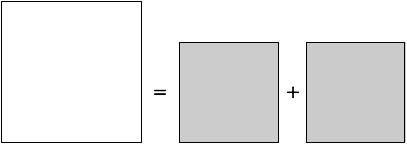
\includegraphics[scale=0.4]{FiguresArithmetic/sqrt2initial}
\caption{{\it A geometric depiction of the Pythagorean Theorem and its
    underlying equation: $a^2 = b^2 + b^2$.}
\label{fig:irrationality1}}
\end{center}
\end{figure}
suggestively invokes the Pythagorean Theorem.  The figure displays
three squares: The two small grey squares are identical, with common
area $A$, while the large white square has double this area.  By the
Pythagorean Theorem, if the small squares have (common) side-lengths
$b \in \N^+$, hence share area $A = b^2$ each, then the large square
has side-lengths $a \eqdef \sqrt{2}b$, hence has area $a^2 = 2 b^2$.

As in the classical proof, in
Section~\ref{sec:classical-proof-sqrt(2)}, we now assume that
$\sqrt{2}$ is rational.  Within the context of
Fig.~\ref{fig:irrationality1}, this means that
\[ \sqrt{2} \ = \ {a \over b} \]
for $a, b \in \N^+$.  Since all that we have said thus far holds for
arbitrary $a$ and $b$, we are free to consider the assumption's
implications for the same situation as before,
%Section~\ref{sec:classical-proof-sqrt(2)}, 
namely, that $a$ and $b$ do
not share any common prime factor.  Note additionally that,
because\footnote{If this inequality is new to you, then just note that
  $(1.4)^2 = 1.96$, which is less than $2$.}
\[ \sqrt{2} \ > \ 1.4, \]
we know that $a > b$.
\medskip

\noindent \fbox{
\begin{minipage}{0.97\textwidth}
Of course, our demands on the relationship between the numerator $a$
and the denominator $b$ lose no generality in our argument.  To wit,
``$\displaystyle {a \over b}$'' is just one name for the depicted
rational number, and choosing any specific name has no impact on the
number itself.
\end{minipage}
}
\medskip

Now that we have the suggestive ``equation'' presented in
Fig.~\ref{fig:irrationality1}, we can manipulate the depicted squares.
Let us embed both of the grey $b \times b$ squares of
Fig.~\ref{fig:irrationality1} into the white $a \times a$ square, in
the overlapped manner depicted in Fig.~\ref{fig:irrationality2}:
\begin{figure}[htb]
\begin{center}
       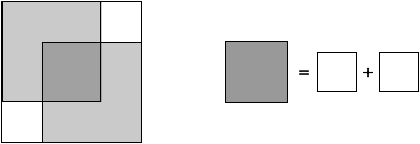
\includegraphics[scale=0.4]{FiguresArithmetic/sqrt2final}
\caption{{\it Construction of a smaller pythagorian equation.}
\label{fig:irrationality2}}
\end{center}
\end{figure}
one grey square is nestled into the northwestern corner of the white
square, while the other is nestled into the southeastern corner.
The overlapping of the grey squares under this
embedding creates a new square---depicted in dark grey---in the center
of the white square, while it leaves unoccupied two small squares,
which remain white in the figure.

Now, let us get quantitative.
\begin{itemize}
\item
On the one hand, the fact that the combined areas of the two grey
squares equal the area of the white square guarantees that the area of
the dark grey overlap-square is equal to the combined areas of the
small unoccupied white squares.

\item
On the other hand, because the side-length of the large white square
is $a$, while the (common) side-length of the grey squares is $b$, it
follows that the side-lengths of the small white square is $a-b$, and
the side-length of the dark grey overlap-square is $2b-a$.  All of
these side-lengths are positive because of the value of $\sqrt{2}$.
To wit: ($i$) $a > b$ because $\sqrt{2} >1$; ($ii$) $2b >a$ because
$\sqrt{2} < 2$.
\end{itemize}
The preceding facts allow us to label the squares of
Fig.~\ref{fig:irrationality1} differently than we did earlier---and
derive a different valid ``equation''.  As we did at the beginning of
this discussion, we again invoke the Pythagorian Theorem, but now we
do so while focusing---cf., Fig.~\ref{fig:irrationality2}---on the
dark grey overlap-square (which plays the role of the large square in
Fig.~\ref{fig:irrationality1}) and the two small white squares (which
play the role of the two small squares in
Fig.~\ref{fig:irrationality1}).  Whereas our original focus led to the
putative rational value $\displaystyle {a \over b}$ for $\sqrt{2}$,
the new focus yields the putative rational value $\displaystyle {2b-a
  \over a-b}$ for $\sqrt{2}$.  We thus have
\[ \sqrt{2} \ = \ {a \over b} \ = \ {2b-a \over a-b}, \]
where $2b-a \ < \ a$ and $a-b \ < \ b$.  In the light of the
Fundamental Theorem of Arithmetic (Theorem~\ref{thm:Fund-Thm-Arith}),
this new rational name for $\sqrt{2}$ contradicts our starting
assumption that $\displaystyle {a \over b}$ was a fration in lowest
terms, i.e., in which $a$ and $b$ share no common factor. % is the simplest name.
\qed
\end{proof}

%{\Denis I did not find a better word for simplest...}
%{\Denis I have another geometric proof for the same result,
%I added it in the separate file which will serve as exercices.}


\section{The Basics of the Complex Numbers}
\label{sec:complexes}

Let us denote by $\C$ the set of complex numbers.  Each number $\kappa
= a+bi \in \C$ has a {\it real} \index{number!complex!real part} {\em
  part}---the part that {\em does not} involve the imaginary unit
\index{$i$: the imaginary unit} $i$---and an {\it imaginary}
\index{number!complex!imaginary part} {\em part}---the part that {\em
  does} involve $i$.  To be explicit: the real part of our number
$\kappa$, is \index{complex number!real part Re($\cdot$)} Re$(\kappa)
= a$; the {\it imaginary part} of our number $\kappa$,is
\index{complex number!imaginary part Im($\cdot$)} Im$(\kappa) = b$.
\index{complex number!imaginary part Im($\cdot$)} The notation
Re$(\kappa)$ and Im$(\kappa)$ is common but not universal.

\index{complex number!multiplication!three real multiplications}
Using the basic arithmetic laws that we have discussed thus far, plus
the defining equation, $i^2 = -1$, of the imaginary unit $i$, we find
that the {\em product} of two complex numbers, $a+bi \in \C$ and $c+di
\in \C$ is the complex number, call it $\kappa$,
\begin{equation}
\label{eq:complex-mult}
\kappa \ = \ (a+bi) \cdot (c+di) \ = \ (ac - bd) + (ad + bc)i.
\end{equation}
We note that a ``direct'' implementation of complex multiplication,
i.e., one that implements (\ref{eq:complex-mult}) literally, requires
four real multiplications---namely, $ac, bd, ad, bc$.

During the 1960s, people first began to pay close attention to the
costs associated with various ways of achieving computational results.
They sought---and found---a number of procedures that replaced
computations involving $k$ real multiplications (a relatively
expensive operation) and $\ell$ real additions (a relatively
inexpensive operation) by computations that achieved the same result
but used fewer multiplications and not too many more additions.
Complex multiplication was one of the operations they studied.  Here
is the result.

\begin{prop}
\label{thm:complex-mult-3real}
One can compute the product of two complex numbers using {\em three}
real multiplications rather than four.
\end{prop}

The proof of this result involves arithmetic manipulation that require
``thinking outside the box".  We leave the proof as an exercise.  The main
message of the result is that we should never be lulled into assuming that the way
an arithmetic expression {\em is} written is the way that it {\em has
  to be} written.


\ignore{*********************

\begin{proof}
Although implementing (\ref{eq:complex-mult}) ``directly'' correctly
produces the product $\kappa = (a+bi) \cdot (c+di)$, there is another
implementation that is {\em more efficient}.  Specifically, the
following recipe computes $\kappa$ using only {\em three} real
multiplications instead of the four real multiplications of the
``direct'' implementation.  We begin to search for this recipe by
noting that our immediate goal is to compute both Re$(\kappa) = ac-bd$
and Im$(\kappa) = ad+bc$.  We can accomplish this by computing the
{\em three} real products
\begin{equation}
\label{eq:complex-mult-3a}
(a+b) \cdot (c+d); \ \ \ \ \
ac;  \ \ \ \ \ bd
\end{equation}
and then noting that
\begin{equation}
\label{eq:complex-mult-3b}
\begin{array}{lcl}
\mbox{Im}(\kappa) & = & (a+b) \cdot (c+d) - ac -bd, \\
\mbox{Re}(\kappa) & = & ac -bd
\end{array}
\end{equation}
We thereby achieve the result of the complex multiplication described
in (\ref{eq:complex-mult}) while using only {\em three} real
multiplications.

Of course, a full reckoning of the costs of the two implementations we
have discussed exposes the fact that the implementation that invokes
(\ref{eq:complex-mult-3a}) and (\ref{eq:complex-mult-3b}) uses {\em
  three} real additions rather than the {\em two} real additions of
the ``direct'' implementation.  But this entire exercise was
predicated on the observation that each real addition is much less
costly than a real multiplication, so trading one multiplication for
one addition is an unqualified ``win''.  \qed
\end{proof}

{\Denis I added a sentence to refer to an exercice dealing with karatsuba which uses the same idea...}
Notice that this technique is classical and it has been used in many other situations.
For instance while multiplying two integers in base 2 (see exercice~\ref{Karatsuba}).

*******************}
